\documentclass[UTF-8, a4paper, zihao=-4, no-math, openany, oneside]{ctexbook}

\usepackage{xeCJK}
\usepackage{fontspec}
\usepackage{newtxmath}
\usepackage{fancyhdr}
\usepackage[hmargin=3.2cm, vmargin=3.8cm, footnotesep=1cm]{geometry}
\usepackage{titletoc}

\usepackage{graphicx}
\usepackage[caption=false, font=footnotesize]{subfig}
\usepackage{tabularx}
\usepackage{booktabs}
\usepackage{float}
\usepackage{caption}

\usepackage{amsmath}	
\usepackage{bm}	

\usepackage[numbers, sort, super, square]{natbib}

\usepackage{url}
\usepackage{pifont}
\usepackage[colorlinks=true, bookmarks=true, bookmarksnumbered=true,% 
linkcolor=black, anchorcolor=black, citecolor=black, urlcolor=black]{hyperref}

\setCJKmainfont[AutoFakeBold = true]{SimSun}
\setmainfont{Times New Roman}
\linespread{1.388888888889}
\setlength{\parskip}{0bp}
\raggedbottom

\pagestyle{fancy}
\fancyhf{}
\fancyhead[C]{\small\leftmark}
\fancyfoot[C]{\small\thepage}
\renewcommand{\headrulewidth}{0.4bp} 				
\renewcommand{\footrulewidth}{0bp}

\titlecontents{chapter}[0em]{\linespread{1}\selectfont\vspace*{6bp}}{\thecontentslabel\hspace*{1em}}{}{\titlerule*[0.5pc]{$\cdot$}\contentspage\hspace*{0em}}
\titlecontents{section}[3em]{\linespread{1}\selectfont\vspace*{6bp}}{\thecontentslabel\hspace*{1em}}{}{\titlerule*[0.5pc]{$\cdot$}\contentspage\hspace*{0em}}
\titlecontents{subsection}[5em]{\linespread{1}\selectfont\vspace*{6bp}}{\thecontentslabel\hspace*{1em}}{}{\titlerule*[0.5pc]{$\cdot$}\contentspage\hspace*{0em}}

\renewcommand{\arraystretch}{1.3}
\newcolumntype{Y}{>{\centering\arraybackslash}X}

\makeatletter
\newcommand\dlmu[2][4cm]{\hskip1pt\underline{\hb@xt@ #1{\hss#2\hss}}\hskip3pt}
\makeatother

\newcommand{\cmark}{\ding{51}}%
\newcommand{\xmark}{\ding{55}}%
\newcommand{\done}{\rlap{$\square$}{\raisebox{2pt}{\large\hspace{1pt}\cmark}}\hspace{-1.5pt}}
\newcommand{\wontfix}{\rlap{$\square$}{\large\hspace{10pt}}}

\captionsetup{font=small, labelsep=quad, format=hang, skip=0bp}
\setlength{\abovecaptionskip}{6bp}
\setlength{\belowcaptionskip}{6bp}

\ctexset{
	chapter = {
		number = \thechapter,
		format = {\heiti\bfseries\centering\fontsize{16bp}{19.2bp}\selectfont},
		aftername = {\hspace*{1em}},
		beforeskip = 0bp,
		afterskip = 18bp,
		pagestyle = fancy
	},
	section = {
		format = {\heiti\raggedright\fontsize{14bp}{16.8bp}\selectfont}, 
		aftername = {\hspace*{1em}},
		beforeskip = 24bp, 
		afterskip = 6bp
	},
	subsection = {
		format = {\heiti\fontsize{13bp}{15.6bp}\selectfont}, 
		aftername = {\hspace*{1em}},
		beforeskip = 12bp, 
		afterskip = 6bp
	}
}

\begin{document}
	
\begin{titlepage}

\begin{flushleft}
	
{\heiti 分类:\hfill 密级:\hspace*{6em}}

U D C:\hfill {\heiti 学号:}\hspace*{6em}

\end{flushleft}\vspace*{6ex}
	
\begin{center}

{\heiti \fontsize{16bp}{19.2bp}\selectfont 南\hspace*{0.5em}昌\hspace*{0.5em}大\hspace*{0.5em}学\hspace*{6em}*\hspace*{0.5em}士\hspace*{0.5em}研\hspace*{0.5em}究\hspace*{0.5em}生}\vspace*{4ex}
	
{\heiti \fontsize{24bp}{28.8bp}\selectfont 学位论文}\vspace*{6ex}
	
{\heiti \fontsize{18bp}{21.6bp}\selectfont 南昌大学研究生学位论文\LaTeX 模板}
	
\textbf{\fontsize{14bp}{16.8bp}\selectfont \LaTeX \; Template for Degree Thesis of Nanchang University}\vspace*{6ex}
	
{\fontsize{14bp}{16bp}\selectfont **}

\end{center}

\begin{flushleft}

培\hspace*{0.22em}养\hspace*{0.22em}单\hspace*{0.22em}位\hspace*{0.22em} (院、\hspace*{0.21em}系):信息工程学院\hspace*{1em}计算机系

指导教师姓名、职称:***\hspace*{1em}

申请学位的学科门类:***

学\hspace*{0.6em}科\hspace*{0.6em}专\hspace*{0.6em}业\hspace*{0.6em}名\hspace*{0.6em}称:

论\hspace*{0.6em}文\hspace*{0.6em}答\hspace*{0.6em}辩\hspace*{0.6em}日\hspace*{0.6em}期:\today

\end{flushleft}\vspace*{6ex}

\begin{flushright}
	
答辩委员会主席:\dlmu[6em]{}

评阅人:\dlmu[6em]{}

\dlmu[6em]{}

\dlmu[6em]{}

\end{flushright}\vspace*{6ex}

\begin{center}	
\today
\end{center}

\end{titlepage}	

\frontmatter
\pagenumbering{Roman}

\chaptermark{声明和授权书}
\begin{figure}[H]
\centering
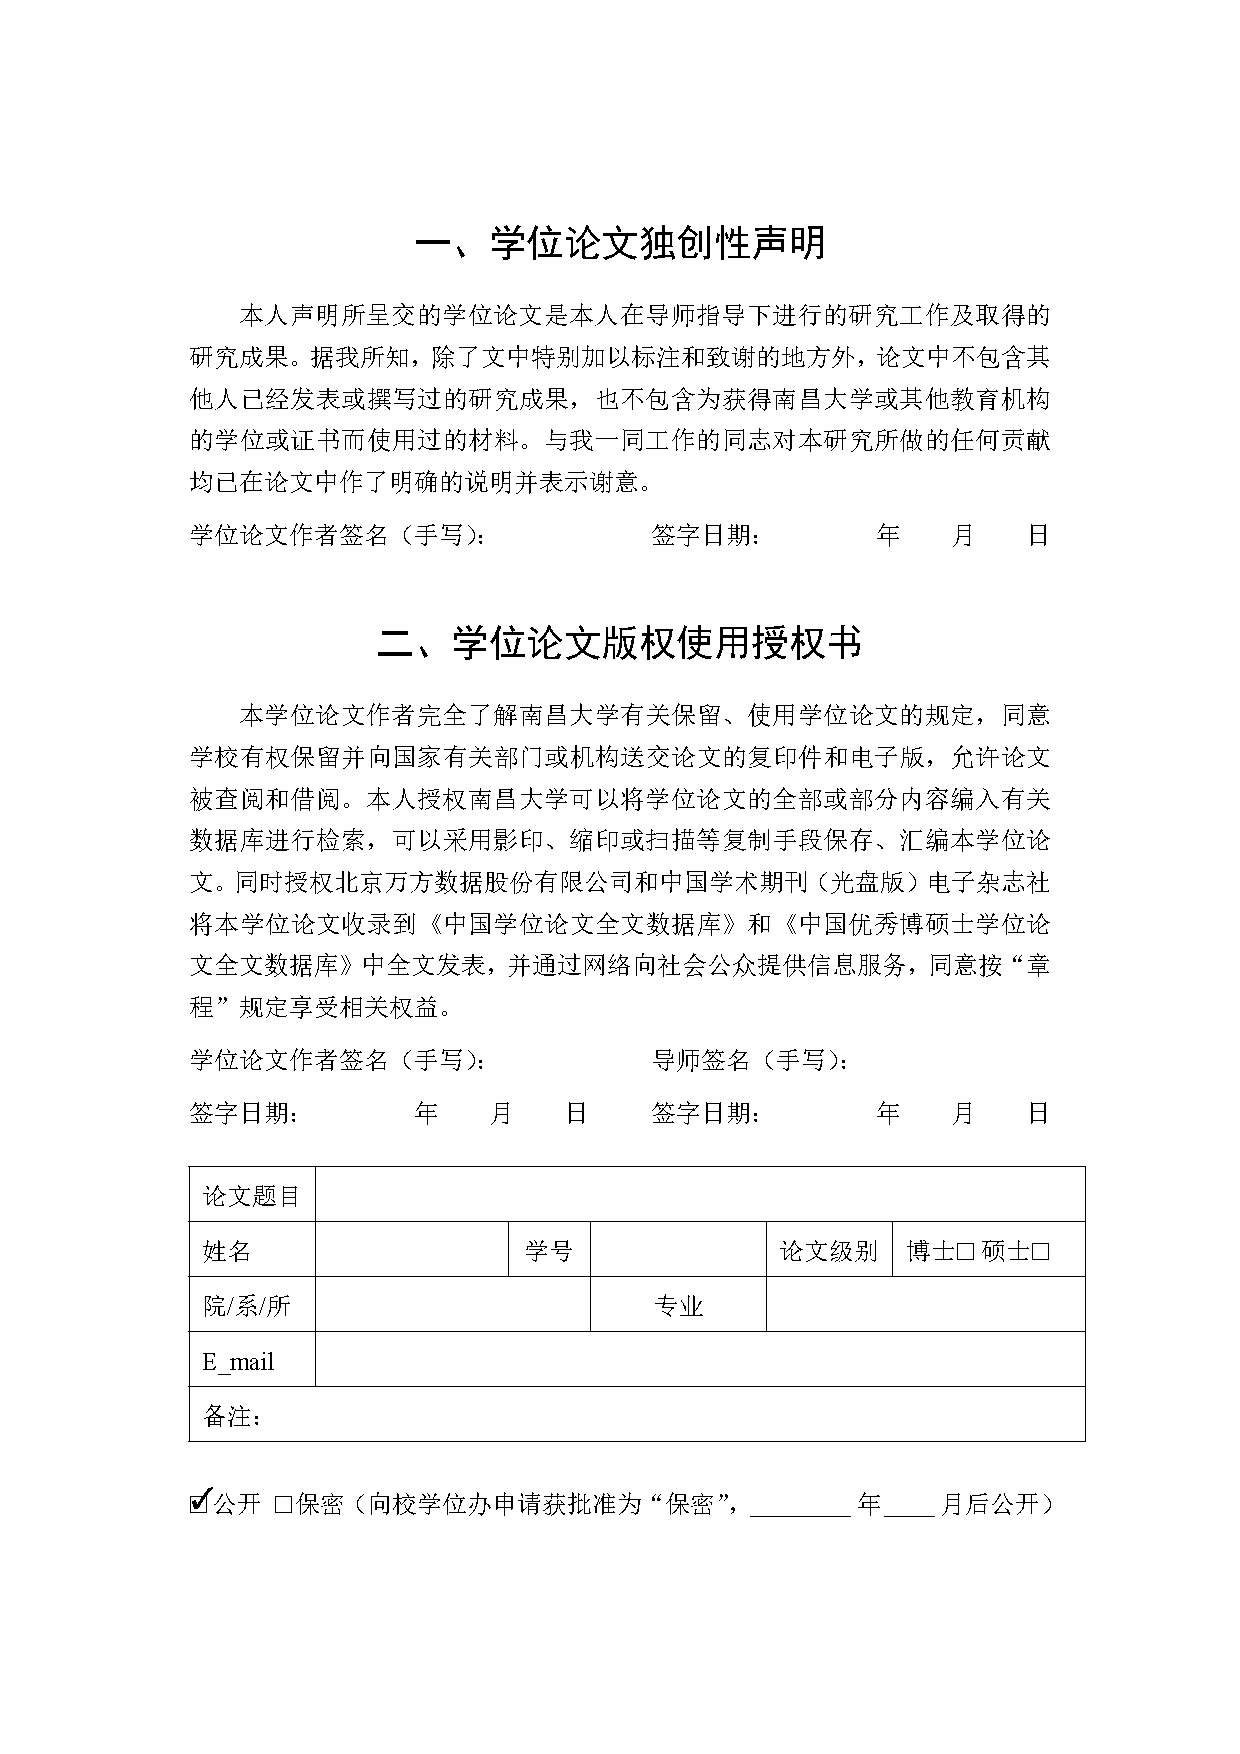
\includegraphics[width=\textwidth]{degree_thesis_declarations_authorizations}
\end{figure}

\clearpage
\pdfbookmark[0]{摘要}{chineseAbstract}
\chapter*{摘要}\chaptermark{摘要}

\vspace*{1ex}\noindent \textbf{关键词:}

\clearpage
\pdfbookmark[0]{ABSTRACT}{abstract}
\chapter*{ABSTRACT}\chaptermark{ABSTRACT}

\vspace*{1ex}\noindent \textbf{Key Words: }

\tableofcontents

\mainmatter
\pagenumbering{arabic}

\chapter{章标题}\label{chapter1}

\section{一级节标题}\label{sec1.1}

\subsection{二级节标题}\label{sec1.1.1}

此\LaTeX 模板由南昌大学在读硕士研究生朱梦编写,欢迎使用,有任何问题可以在我的gitup上留言。同时,希望志同道合的朋友一起维护。希望此\LaTeX 模板能作为南昌大学学位论文的官方选择之一。

\backmatter
\chapter{致谢}

\linespread{1.11111111111112}\selectfont 


\bibliographystyle{gbt7714}
\fontsize{10.5bp}{16bp}\selectfont
\phantomsection
\bibliography{refs}\addcontentsline{toc}{chapter}{参考文献}

\appendix
\chapter{攻读学位期间的研究成果}

\fontsize{10.5bp}{16bp}\selectfont

\end{document}